% Created 2021-03-02 Tue 15:04
% Intended LaTeX compiler: pdflatex
\documentclass[presentation]{beamer}
\usepackage[utf8]{inputenc}
\usepackage[T1]{fontenc}
\usepackage{graphicx}
\usepackage{grffile}
\usepackage{longtable}
\usepackage{wrapfig}
\usepackage{rotating}
\usepackage[normalem]{ulem}
\usepackage{amsmath}
\usepackage{textcomp}
\usepackage{amssymb}
\usepackage{capt-of}
\usepackage{hyperref}
\usetheme[height=20pt]{Rochester}
\author{Shane Mulligan \\  }
\date{\textit{<2021-03-01 Mon>}}
\title{Presenting\ldots{} \\   \emph{\alert{Prompt Engineering in Emacs}} \\  }
\hypersetup{
 pdfauthor={Shane Mulligan \\  },
 pdftitle={Presenting\ldots{} \\   \emph{\alert{Prompt Engineering in Emacs}} \\  },
 pdfkeywords={},
 pdfsubject={},
 pdfcreator={Emacs 27.0.91 (Org mode 9.3)}, 
 pdflang={English}}
\begin{document}

\maketitle

\section{Presentation}
\label{sec:org1de4b6e}
\begin{frame}[label={sec:org77f1fc9},fragile]{Following along}
 \begin{block}{Repositories for following along}
{\footnotesize
\begin{center}
\begin{tabular}{l}
\url{http://github1s.com/semiosis/examplary}\\
\url{http://github1s.com/semiosis/pen.el}\\
\url{http://github1s.com/semiosis/prompts}\\
\url{http://github1s.com/semiosis/prompt-engineering-patterns}\\
\url{http://github1s.com/minimaxir/gpt-3-client}\\
\end{tabular}
\end{center}
}

{\footnotesize
\uline{\alert{slides}}
\begin{center}
\begin{tabular}{l}
\url{http://github1s.com/semiosis/presentation-prompt-engineering-in-emacs}\\
\end{tabular}
\end{center}
}

{\footnotesize
\uline{\alert{glossary}}
\begin{center}
\begin{tabular}{l}
\url{http://github1s.com/mullikine/glossaries-gh/blob/master/openai.txt}\\
\end{tabular}
\end{center}
}
\end{block}

\begin{block}{Demo}
{\footnotesize
\begin{verbatim}
1  ssh -oBatchMode=no shane@124.197.60.232 -p 9922
\end{verbatim}
}
\end{block}
\end{frame}

\section{Preliminaries}
\label{sec:orga26b420}
\subsection{GPT-3}
\label{sec:orgb66f2b7}
\begin{frame}[label={sec:orgf49f62f},fragile]{Text Generator}
 \begin{block}{Background knowledge}
{\footnotesize
\begin{itemize}
\item \texttt{GPT-3} is a \texttt{seq2seq} model (a text generator)
\begin{itemize}
\item It's stochastic but can be configured to be deterministic.
\end{itemize}
\end{itemize}
}
\end{block}

\begin{block}{Key concepts}
{\footnotesize
\begin{itemize}
\item prompt,
\item completion, and
\item tokens
\end{itemize}
}
\end{block}

\begin{block}{Limitations}
{\footnotesize
Combined, the text prompt and generated
completion must be below 2048 tokens (roughly
\textasciitilde{}1500 words).

\begin{description}
\item[{context-stuffing}] With only 2048 tokens, you need to make
use of your real estate by providing
instructions and making implicit
information explicit.
\end{description}
}
\end{block}
\end{frame}

\subsection{A new programming paradigm}
\label{sec:orgc50dd77}
\begin{frame}[label={sec:org6d0979e},fragile]{Prompt Engineering}
 \begin{block}{Characteristics}
{\footnotesize
\begin{itemize}
\item declarative, like \texttt{html}
\item stochastic, like \texttt{problog}
\item Unlocks new types of applications
\item Speeds up development
\end{itemize}
}
\end{block}
\end{frame}

\begin{frame}[label={sec:orged051aa},fragile]{Some prompts I've made}
 \begin{block}{\texttt{generate-vim-command.prompt}}
{\footnotesize
\begin{verbatim}
 1  Vim
 2  
 3  Insert "Q: " at the start of the line
 4  :%s/^/Q: /g.
 5  ###
 6  Remove whitespace from the start of each line
 7  :%s/^\s*/\1/g
 8  ###
 9  Join each line with the next line
10  :1,$j
11  ###
12  Make all occurrences of Steve lowercase
13  :%s/Steve/steve/g
14  ###
15  <1>
\end{verbatim}
}
\end{block}
\end{frame}

\begin{frame}[label={sec:org1312935}]{Tasks suitable for GPT-3}
\begin{block}{Classification}
\begin{itemize}
\item Tweet Sentiment
\item Company categorization
\item Labeling parts of speech
\end{itemize}

{\footnotesize
\begin{itemize}
\item \url{http://github.com/semiosis/prompts/blob/master/prompts/tweet-sentiment-classifier.prompt}
\item \url{http://github.com/semiosis/prompts/blob/master/prompts/keyword-extraction.prompt}
\end{itemize}
}
\end{block}
\end{frame}

\begin{frame}[label={sec:org122def8}]{Tasks suitable for GPT-3}
\begin{block}{Generation}
\begin{itemize}
\item Idea Generator
\end{itemize}

Come up with silly inventions.

\begin{center}
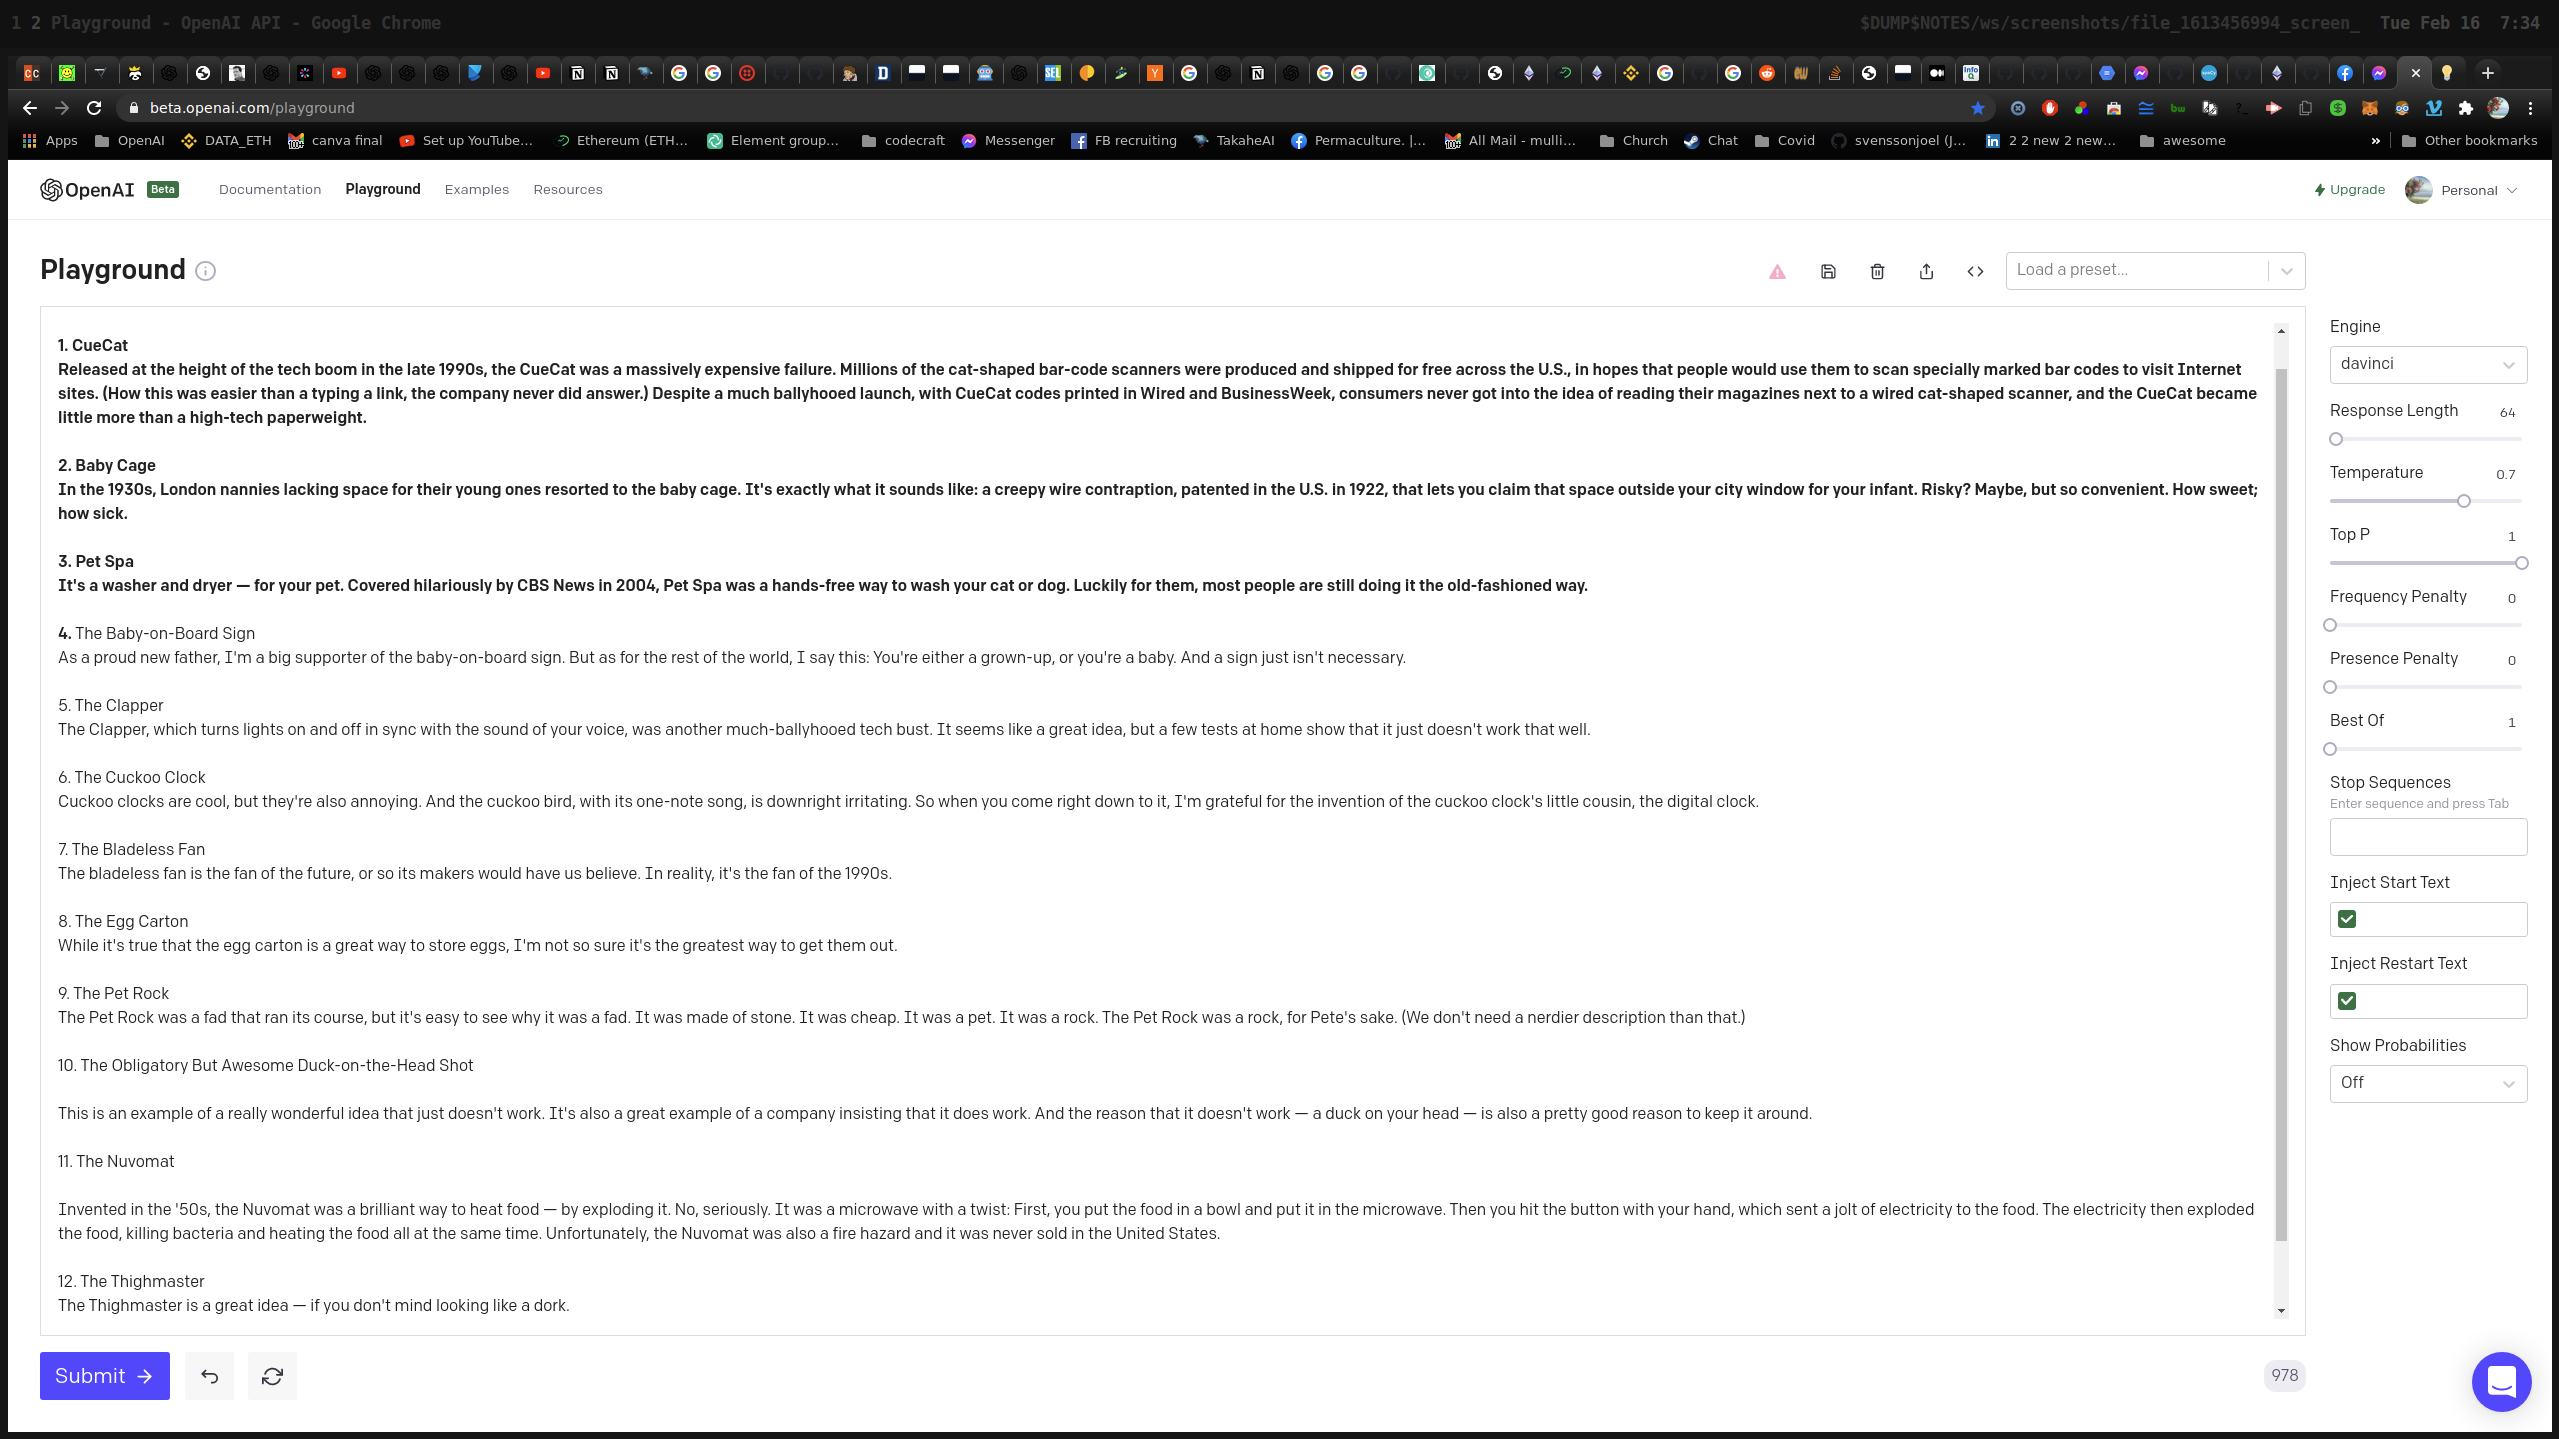
\includegraphics[width=.9\linewidth]{./silly-inventions.png}
\end{center}
\end{block}
\end{frame}

\begin{frame}[label={sec:org1e940f2}]{Tasks suitable for GPT-3}
\begin{block}{Conversation}
\begin{itemize}
\item Q\&A agent
\item Sarcastic chatbot
\end{itemize}

{\footnotesize
\url{http://github.com/semiosis/prompts/blob/master/prompts/sarcastic-response.prompt}
}
\end{block}
\end{frame}

\begin{frame}[label={sec:org12ffa72},fragile]{Design patterns}
 Taken from Prompt Design 101.

These are manual techniques which should be
encoded in a DSL when generating prompts.

\begin{block}{1. Reflective description of the task}
State what the prompt does at the start At the
start of the example we state in plain
language what the classifier does:

\begin{verbatim}
1  _This is a tweet sentiment classifier._
\end{verbatim}

By stating this up front

it helps the API understand much more quickly
what the goal of the response is supposed to
be

and you’ll end needing to provide fewer
examples.
\end{block}
\end{frame}

\begin{frame}[label={sec:org1d2e5c9},fragile]{Design patterns}
 Taken from Prompt Design 101.

These are manual techniques which should be
encoded in a DSL when generating prompts.

\begin{block}{2. Use separators between examples}
Example: \texttt{\#\#\#}.

You can use other characters or line breaks,
but \texttt{\#\#\#} works pretty consistently and is
also an easy to use stop sequence.

Whatever separator you use, make sure that
it’s clear to the API where an example starts
and stops.
\end{block}
\end{frame}

\begin{frame}[label={sec:org187ede6},fragile]{Design patterns}
 Taken from Prompt Design 101.

These are manual techniques which should be
encoded in a DSL when generating prompts.

\begin{block}{Improving the classifier’s efficiency Part 1}
Make a prompt more efficient / cheaper.

Design it to generate multiple results from
one API call.

{\footnotesize
\begin{verbatim}
 1  This is a tweet sentiment classifier
 2  Tweet: "I loved the new Batman movie!"
 3  Sentiment: Positive
 4  ###
 5  Tweet: "I hate it when my phone battery dies"
 6  Sentiment: Negative
 7  ###
 8  Tweet: "My day has been 👍"
 9  Sentiment: Positive
10  ###
11  Tweet: "This is the link to the article"
12  Sentiment: Neutral
13  ###
14  Tweet text
\end{verbatim}

}
\end{block}
\end{frame}

\begin{frame}[label={sec:org2740d82},fragile]{Design patterns}
 Taken from Prompt Design 101.

These are manual techniques which should be
encoded in a DSL when generating prompts.

\begin{block}{Improving the classifier’s efficiency Part 2}
{\footnotesize
\begin{verbatim}
 1  1. "I loved the new Batman movie!"
 2  2. "I hate it when my phone battery dies"
 3  3. "My day has been 👍"
 4  4. "This is the link to the article"
 5  5. "This new music video blew my mind"
 6  
 7  Tweet sentiment ratings:
 8  1: Positive
 9  2: Negative
10  3: Positive
11  4: Neutral
12  5: Positive
13  
14  ###
15  Tweet text
\end{verbatim}
}
\end{block}
\end{frame}

\begin{frame}[label={sec:orgf64a35b},fragile]{Design patterns}
 Taken from Prompt Design 101.

These are manual techniques which should be
encoded in a DSL when generating prompts.

\begin{block}{Improving the classifier’s efficiency Part 3}
{\footnotesize
\begin{verbatim}
1  "I can't stand homework"
2  "This sucks. I'm bored 😠"
3  "I can't wait for Halloween!!!"
4  "My cat is adorable ❤️❤️"
5  "I hate chocolate"
6  Tweet sentiment ratings:
7  1.
\end{verbatim}
}
\end{block}
\end{frame}

\begin{frame}[label={sec:org07b2985}]{Techniques}
\begin{block}{Query Reformulation}
\url{https://www.sciencedirect.com/topics/computer-science/query-reformulation}

You can improve the quality of the responses
by making a longer more diverse list in your
prompt.

One way to do that is to start off with one
example, let the API generate more and select
the ones that you like best and add them to
the list.

A few more high-quality variations can
dramatically improve the quality of the
responses.
\end{block}
\end{frame}

\section{Explanations}
\label{sec:org2da5cec}
\subsection{Using \texttt{pen.el}}
\label{sec:orgf63788d}
\begin{frame}[label={sec:org80b5331},fragile]{Prompt YAML format Part 1}
 \begin{block}{\texttt{meeting-bullets-to-summary.prompt}}
\begin{verbatim}
 1  title: "meeting bullet points to summary"
 2  prompt: |+
 3      Convert my short hand into a first-hand
 4      account of the meeting:
 5  
 6      <1>
 7  
 8      Summary:
 9  engine: "davinci-instruct-beta"
10  temperature: 0.7
11  max-tokens: 60
\end{verbatim}
\end{block}
\end{frame}

\begin{frame}[label={sec:org5329f57},fragile]{Prompt YAML format Part 2}
 \begin{block}{\texttt{meeting-bullets-to-summary.prompt}}
\begin{verbatim}
1  top-p: 1
2  frequency-penalty: 0.0
3  presence-penalty: 0.0
4  best-of: 1
5  stop-sequences:
6  - "\n\n"
7  conversation-mode: no
8  stitch-max: 0
\end{verbatim}

\begin{description}
\item[{stitch-max}] Keep stitching together until reaching this limit.
This allows a full response for answers which may need n*max-tokens to reach the stop-sequence.
\end{description}
\end{block}
\end{frame}

\begin{frame}[label={sec:org6cfb005},fragile]{Prompt YAML format: Part 3}
 \begin{block}{\texttt{meeting-bullets-to-summary.prompt}}
\begin{verbatim}
1  vars:
2  - "notes"
3  examples:
4  - |+
5      Tom: Profits up 50%
6      Jane: New servers are online
7      Kjel: Need more time to fix software
8      Jane: Happy to help
9      Parkman: Beta testing almost done
\end{verbatim}
\end{block}
\end{frame}

\section{\texttt{semiosis}}
\label{sec:orgce9344c}
\subsection{\texttt{pen.el}}
\label{sec:orgb706915}
\begin{frame}[label={sec:org9d6cdf2},fragile]{\texttt{Prompts as functions}}
 \begin{block}{\texttt{pen-generate-prompt-functions}}
Generate prompt functions for the files in the
prompts directory Function names are prefixed
with \texttt{pen-pf-} for easy searching.

\url{http://github.com/semiosis/prompts}
\end{block}
\end{frame}

\subsection{\texttt{examplary}}
\label{sec:orgab07308}
\begin{frame}[label={sec:orgf33a573},fragile]{\texttt{examplary}: examples as functions}
 An example-oriented DSL that can be used to
construct and compose NLP tasks.

Why is a DSL needed for this? Just to make the
code a little more terse.

\begin{block}{Regex}
\url{https://github.com/pemistahl/grex}

{\footnotesize
\begin{verbatim}
1  (def regex
2    "example 1\nexample2" "^example [12]$"
3    "example 2\nexample3" "^example [23]$"
4    "pi4\npi5" "^pi[45]$")
\end{verbatim}
}
\end{block}
\end{frame}

\begin{frame}[label={sec:org5adca77},fragile]{\texttt{examplary}: examples as functions}
 \begin{block}{Analogy}
{\footnotesize
\begin{verbatim}
 1  (def analogy
 2    ;; Each line is a training example.
 3    "NNs" "NNs are like genetic algorithms in
 4    that both are systems that learn from
 5    experience"
 6    "Social media" "Social media is like a
 7    market in that both are systems that
 8    coordinate the actions of many
 9    individuals.")
10  
11  (def field
12    "chemistry" "study of chemicals"
13    "biology" "study of living things")
\end{verbatim}
}
\end{block}
\end{frame}

\section{Demonstrations}
\label{sec:orgf081774}
\begin{frame}[label={sec:org8cf329d}]{Something funny}
\begin{block}{Vexate a simple instruction}
\begin{center}
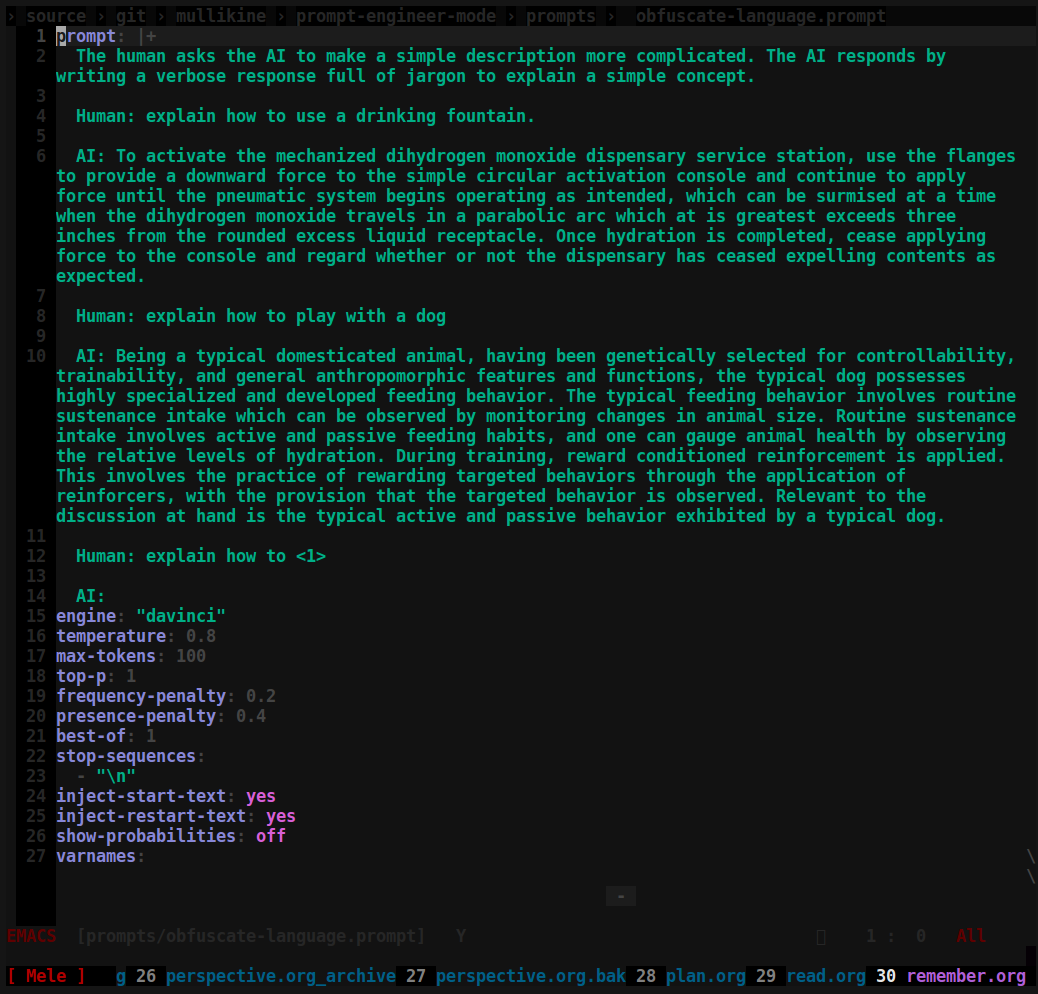
\includegraphics[width=.9\linewidth]{./complicate.png}
\end{center}
\end{block}
\end{frame}

\begin{frame}[label={sec:org06a501b}]{Something funny}
\begin{block}{How to crack an egg}
\begin{center}
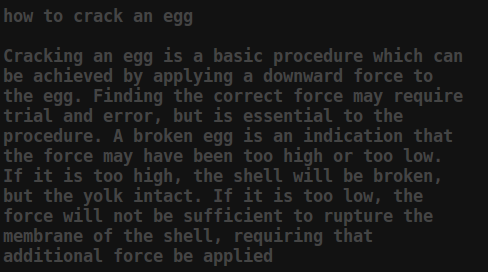
\includegraphics[width=.9\linewidth]{./crack-an-egg.png}
\end{center}
\end{block}
\end{frame}

\begin{frame}[label={sec:org24f3bc3}]{Create a prompt}
\begin{block}{Ask the audience}
\begin{itemize}
\item What type of text to generate
\begin{itemize}
\item Could be code, prose, etc.
\end{itemize}
\end{itemize}
\end{block}
\end{frame}

\section{Appendix}
\label{sec:orga21c342}
\subsection{Additional reading}
\label{sec:orgde7e3ab}
\begin{frame}[label={sec:orga8240fe}]{Tutorials}
\begin{block}{Ruby}
{\footnotesize
\url{https://www.twilio.com/blog/generating-cooking-recipes-openai-gpt3-ruby}
}
\end{block}
\end{frame}
\end{document}
